We brively recall the definitions of hypergraphs from~\cite{plump2018modular}.
Intuitively, a hypergraph is a mathematical structure consisting of a set of nodes and a set of hyperedges, where nodes and hyperedges are labelled. Each hyperedge can connect any number of nodes which form a finite sequences of nodes. The label of a hyperedge decides the number of nodes it connects and the labels of the nodes.
\begin{definition}[Signature of a hypergraph~\cite{plump2018modular}]
    A signature $\Sigma = \langle \Sigma_V, \Sigma_E, \text{Type} \rangle$ consists of 
    \begin{itemize}
        \item a set $\Sigma_V$ of node labels,
        \item a set $\Sigma_E$ of hyperedge labels, and
        \item a function $\text{Type}$ assigning to each $l \in \Sigma_E$ a set of strings $\text{Type}(l) \subseteq \Sigma_V^*$.
    \end{itemize}
\end{definition}
Unless stated otherwise, we denote by $\Sigma$ an arbitrary but fixed signature over which all hypergraphs are labelled.
\begin{remark}
    The extension $f^* : A^* \to B^*$ of a function $f : A \to B$ maps the empty string to itself and $a_1 \ldots a_n$ to $f(a_1) \ldots f(a_n)$.
\end{remark}
\begin{definition}[Hypergraph~\cite{plump2018modular}]
    A hypergraph over $\Sigma$ is a system $G = \langle V_G, E_G, \text{mark}_G, \text{lab}_G, \text{att}_G \rangle$ consisting of 
    \begin{itemize}
        \item a finite set $V_G$ of nodes,
        \item a finite set $E_G$ of hyperedges,
        \item two labelling functions $\text{mark}_G : V_G \to \Sigma_V$ and $\text{lab}_G : E_G \to \Sigma_E$, and
        \item an attachment function $\text{att}_G : E_G \to V_G^*$ such that $\text{mark}_G^*(\text{att}_G(e)) \in \text{Type}(\text{lab}_G(e))$ for each hyperedge $e$.
    \end{itemize} 
\end{definition} 

\begin{example}
    We adopt the notation from~\cite[\textsection 2.1]{plump2018modular} to visualize hypergraphs. \enquote{nodes and hyperedges are drawn as circles and boxes, respectively, with labels inside. Lines represent the attachment of hyperedges to nodes, where numbers specify the left-to-right order in the attachment string.} The following shows a hypergraph with three nodes all labeled with $\epsilon$ and three hyperedges (labeled with $s$ and $0$).

    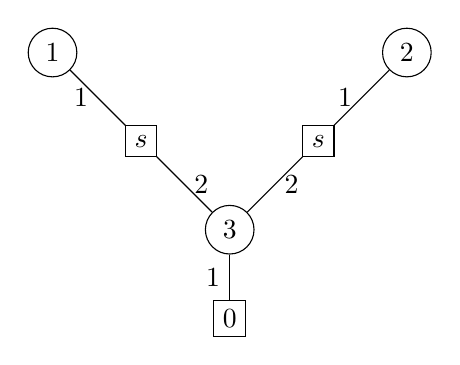
\begin{tikzpicture}[scale=0.75]
        \node[draw,circle] (n1) at (-3,3) {1};
        \node[draw,circle] (n2) at (3,3) {2};
        \node[draw,circle] (n3) at (0,0) {3};
        \node[draw,rectangle] (e1) at (-1.5,1.5) {$s$};
        \node[draw,rectangle] (e2) at (1.5,1.5) {$s$};
        \node[draw,rectangle] (e3) at (0, -1.5) {0};
        \draw (e1) -- (n1) node[midway,left] {1};
        \draw (e1) -- (n3) node[midway,right] {2};
        \draw (e2) -- (n2) node[midway,left] {1};
        \draw (e2) -- (n3) node[midway,right] {2};
        \draw (e3) -- (n3) node[midway,left] {1};
    \end{tikzpicture}
\end{example}

\begin{definition}[Hypergraph homomorphism~\cite{plump2018modular}]
    Give hypergraphs $G$ and $H$, a hypergraph homomorphism $h : G \to H$ consists of functions $h_V : V_G \to V_H$ and $h_E : E_G \to E_H$ that preserve labels and attachment to nodes, i.e., $\opn{mark}_H \circ h_V = \opn{mark}_G$ and $\opn{lab}_H \circ h_E = \opn{lab}_G$ and $\opn{att}_H \circ h_E = g_V \circ \opn{att}_G$.
\end{definition}